%% Supplementary file. Scientific legends are placeholders.
%% The AI-use log below is a formal statement for the author to review.
\ifdefined\pdfminorversion
  \pdfminorversion=5
\fi
\documentclass[unnumsec,webpdf,contemporary,large,namedate]{oup-authoring-template}
\usepackage{booktabs}
\graphicspath{{../figures/}}
\newcommand{\societylogo}{}
% Generated by scripts/cellbridge_numbers_v100.py. Do not edit by hand.
\newcommand{\Num}[1]{#1}
\newcommand{\NGseTrain}{11}
\newcommand{\NGseCal}{9}
\newcommand{\NGseTest}{10}
\newcommand{\NEmTrain}{64}
\newcommand{\NEmCal}{31}
\newcommand{\NEmTest}{29}
\newcommand{\MaeGseCbEone}{0.284}
\newcommand{\MaeGseCbEtwo}{0.322}
\newcommand{\MaeGseAbEone}{0.315}
\newcommand{\MaeGseAbEtwo}{0.359}
\newcommand{\MaeGseTvEone}{0.393}
\newcommand{\MaeGseTvEtwo}{0.395}
\newcommand{\MaeGseRoEone}{0.376}
\newcommand{\MaeGseRoEtwo}{0.461}
\newcommand{\MaeGseJtEone}{0.756}
\newcommand{\MaeGseJtEtwo}{0.722}
\newcommand{\MaeGseRnEone}{0.799}
\newcommand{\MaeGseRnEtwo}{0.755}
\newcommand{\MaeGseMnEone}{0.511}
\newcommand{\MaeGseMnEtwo}{0.643}
\newcommand{\MaeEmCbEone}{0.530}
\newcommand{\MaeEmCbEtwo}{0.471}
\newcommand{\MaeEmAbEone}{0.526}
\newcommand{\MaeEmAbEtwo}{0.472}
\newcommand{\MaeEmTvEone}{0.929}
\newcommand{\MaeEmTvEtwo}{0.844}
\newcommand{\MaeEmRoEone}{0.889}
\newcommand{\MaeEmRoEtwo}{0.815}
\newcommand{\MaeEmJtEone}{0.889}
\newcommand{\MaeEmJtEtwo}{0.824}
\newcommand{\MaeEmRnEone}{0.889}
\newcommand{\MaeEmRnEtwo}{0.824}
\newcommand{\MaeEmMnEone}{0.889}
\newcommand{\MaeEmMnEtwo}{0.824}
\newcommand{\GseHOneGain}{0.321}
\newcommand{\GseHOneLo}{0.238}
\newcommand{\GseHOneHi}{0.410}
\newcommand{\GseHOneP}{=0.002}
\newcommand{\GseHOneWins}{10}
\newcommand{\GseHOneN}{10}
\newcommand{\GseHOneTested}{tested}
\newcommand{\GseHOneCall}{rejected}
\newcommand{\GseHTwoGain}{0.400}
\newcommand{\GseHTwoLo}{0.158}
\newcommand{\GseHTwoHi}{0.682}
\newcommand{\GseHTwoP}{=0.006}
\newcommand{\GseHTwoWins}{9}
\newcommand{\GseHTwoN}{10}
\newcommand{\GseHTwoTested}{tested}
\newcommand{\GseHTwoCall}{rejected}
\newcommand{\GseHThreeGain}{0.432}
\newcommand{\GseHThreeLo}{0.169}
\newcommand{\GseHThreeHi}{0.742}
\newcommand{\GseHThreeP}{=0.006}
\newcommand{\GseHThreeWins}{9}
\newcommand{\GseHThreeN}{10}
\newcommand{\GseHThreeTested}{tested}
\newcommand{\GseHThreeCall}{rejected}
\newcommand{\GseHFourGain}{0.227}
\newcommand{\GseHFourLo}{0.142}
\newcommand{\GseHFourHi}{0.305}
\newcommand{\GseHFourP}{=0.004}
\newcommand{\GseHFourWins}{9}
\newcommand{\GseHFourN}{10}
\newcommand{\GseHFourTested}{tested}
\newcommand{\GseHFourCall}{rejected}
\newcommand{\GseHFiveGain}{0.472}
\newcommand{\GseHFiveLo}{0.198}
\newcommand{\GseHFiveHi}{0.771}
\newcommand{\GseHFiveP}{=0.002}
\newcommand{\GseHFiveWins}{10}
\newcommand{\GseHFiveN}{10}
\newcommand{\GseHFiveTested}{tested}
\newcommand{\GseHFiveCall}{rejected}
\newcommand{\GseHSixGain}{0.516}
\newcommand{\GseHSixLo}{0.218}
\newcommand{\GseHSixHi}{0.846}
\newcommand{\GseHSixP}{=0.002}
\newcommand{\GseHSixWins}{10}
\newcommand{\GseHSixN}{10}
\newcommand{\GseHSixTested}{tested}
\newcommand{\GseHSixCall}{rejected}
\newcommand{\GseHSevenGain}{0.072}
\newcommand{\GseHSevenLo}{0.032}
\newcommand{\GseHSevenHi}{0.113}
\newcommand{\GseHSevenP}{=0.010}
\newcommand{\GseHSevenWins}{9}
\newcommand{\GseHSevenN}{10}
\newcommand{\GseHSevenTested}{tested}
\newcommand{\GseHSevenCall}{rejected}
\newcommand{\GseHEightGain}{0.109}
\newcommand{\GseHEightLo}{0.043}
\newcommand{\GseHEightHi}{0.183}
\newcommand{\GseHEightP}{=0.016}
\newcommand{\GseHEightWins}{8}
\newcommand{\GseHEightN}{10}
\newcommand{\GseHEightTested}{tested}
\newcommand{\GseHEightCall}{rejected}
\newcommand{\GseHNineGain}{0.037}
\newcommand{\GseHNineLo}{-0.003}
\newcommand{\GseHNineHi}{0.085}
\newcommand{\GseHNineP}{=0.154}
\newcommand{\GseHNineWins}{7}
\newcommand{\GseHNineN}{10}
\newcommand{\GseHNineTested}{tested}
\newcommand{\GseHNineCall}{not rejected}
\newcommand{\GseHTenGain}{0.032}
\newcommand{\GseHTenLo}{-0.050}
\newcommand{\GseHTenHi}{0.113}
\newcommand{\GseHTenP}{=0.492}
\newcommand{\GseHTenWins}{5}
\newcommand{\GseHTenN}{10}
\newcommand{\GseHTenTested}{not tested in sequence}
\newcommand{\GseHTenCall}{not rejected}
\newcommand{\GseNiEoneUpper}{0.050}
\newcommand{\GseNiEoneHold}{held}
\newcommand{\GseNiEtwoUpper}{0.003}
\newcommand{\GseNiEtwoHold}{held}
\newcommand{\GseCovCb}{0.883}
\newcommand{\EmHOneGain}{0.353}
\newcommand{\EmHOneLo}{0.108}
\newcommand{\EmHOneHi}{0.668}
\newcommand{\EmHOneP}{<0.001}
\newcommand{\EmHOneWins}{21}
\newcommand{\EmHOneN}{29}
\newcommand{\EmHOneTested}{tested}
\newcommand{\EmHOneCall}{rejected}
\newcommand{\EmHTwoGain}{0.353}
\newcommand{\EmHTwoLo}{0.108}
\newcommand{\EmHTwoHi}{0.668}
\newcommand{\EmHTwoP}{<0.001}
\newcommand{\EmHTwoWins}{21}
\newcommand{\EmHTwoN}{29}
\newcommand{\EmHTwoTested}{tested}
\newcommand{\EmHTwoCall}{rejected}
\newcommand{\EmHThreeGain}{0.353}
\newcommand{\EmHThreeLo}{0.108}
\newcommand{\EmHThreeHi}{0.668}
\newcommand{\EmHThreeP}{<0.001}
\newcommand{\EmHThreeWins}{21}
\newcommand{\EmHThreeN}{29}
\newcommand{\EmHThreeTested}{tested}
\newcommand{\EmHThreeCall}{rejected}
\newcommand{\EmHFourGain}{0.359}
\newcommand{\EmHFourLo}{0.032}
\newcommand{\EmHFourHi}{0.780}
\newcommand{\EmHFourP}{=0.061}
\newcommand{\EmHFourWins}{16}
\newcommand{\EmHFourN}{29}
\newcommand{\EmHFourTested}{tested}
\newcommand{\EmHFourCall}{not rejected}
\newcommand{\EmHFiveGain}{0.359}
\newcommand{\EmHFiveLo}{0.032}
\newcommand{\EmHFiveHi}{0.780}
\newcommand{\EmHFiveP}{=0.061}
\newcommand{\EmHFiveWins}{16}
\newcommand{\EmHFiveN}{29}
\newcommand{\EmHFiveTested}{not tested in sequence}
\newcommand{\EmHFiveCall}{not rejected}
\newcommand{\EmHSixGain}{0.359}
\newcommand{\EmHSixLo}{0.032}
\newcommand{\EmHSixHi}{0.780}
\newcommand{\EmHSixP}{=0.061}
\newcommand{\EmHSixWins}{16}
\newcommand{\EmHSixN}{29}
\newcommand{\EmHSixTested}{not tested in sequence}
\newcommand{\EmHSixCall}{not rejected}
\newcommand{\EmHSevenGain}{0.374}
\newcommand{\EmHSevenLo}{0.113}
\newcommand{\EmHSevenHi}{0.707}
\newcommand{\EmHSevenP}{<0.001}
\newcommand{\EmHSevenWins}{21}
\newcommand{\EmHSevenN}{29}
\newcommand{\EmHSevenTested}{not tested in sequence}
\newcommand{\EmHSevenCall}{not rejected}
\newcommand{\EmHEightGain}{0.399}
\newcommand{\EmHEightLo}{0.062}
\newcommand{\EmHEightHi}{0.824}
\newcommand{\EmHEightP}{=0.030}
\newcommand{\EmHEightWins}{18}
\newcommand{\EmHEightN}{29}
\newcommand{\EmHEightTested}{not tested in sequence}
\newcommand{\EmHEightCall}{not rejected}
\newcommand{\EmHNineGain}{0.001}
\newcommand{\EmHNineLo}{-0.028}
\newcommand{\EmHNineHi}{0.029}
\newcommand{\EmHNineP}{=0.931}
\newcommand{\EmHNineWins}{15}
\newcommand{\EmHNineN}{29}
\newcommand{\EmHNineTested}{not tested in sequence}
\newcommand{\EmHNineCall}{not rejected}
\newcommand{\EmHTenGain}{-0.003}
\newcommand{\EmHTenLo}{-0.073}
\newcommand{\EmHTenHi}{0.065}
\newcommand{\EmHTenP}{=0.931}
\newcommand{\EmHTenWins}{14}
\newcommand{\EmHTenN}{29}
\newcommand{\EmHTenTested}{not tested in sequence}
\newcommand{\EmHTenCall}{not rejected}
\newcommand{\EmNiEoneUpper}{0.073}
\newcommand{\EmNiEoneHold}{did not hold}
\newcommand{\EmNiEtwoUpper}{0.028}
\newcommand{\EmNiEtwoHold}{held}
\newcommand{\EmCovCb}{0.926}
\newcommand{\EmStopped}{H4}
\newcommand{\GseClaim}{supported}
\newcommand{\EmClaim}{not supported}
\newcommand{\MetaMnFe}{0.324}
\newcommand{\MetaMnSe}{0.044}
\newcommand{\MetaMnRe}{0.324}
\newcommand{\MetaMnReSe}{0.044}
\newcommand{\MetaJtFe}{0.377}
\newcommand{\MetaJtSe}{0.102}
\newcommand{\MetaJtRe}{0.377}
\newcommand{\MetaJtReSe}{0.102}
\newcommand{\MetaRnFe}{0.391}
\newcommand{\MetaRnSe}{0.106}
\newcommand{\MetaRnRe}{0.391}
\newcommand{\MetaRnReSe}{0.106}
\newcommand{\MetaTvFe}{0.078}
\newcommand{\MetaTvSe}{0.021}
\newcommand{\MetaTvRe}{0.183}
\newcommand{\MetaTvReSe}{0.145}
\newcommand{\MetaAbFe}{0.012}
\newcommand{\MetaAbSe}{0.013}
\newcommand{\MetaAbRe}{0.015}
\newcommand{\MetaAbReSe}{0.017}
\newcommand{\DevCb}{0.777}
\newcommand{\DevAb}{0.896}
\newcommand{\DevJt}{0.985}
\newcommand{\DevRn}{0.988}
\newcommand{\DevMn}{1.032}
\newcommand{\AblFull}{0.777}
\newcommand{\AblAnchor}{0.774}
\newcommand{\AblKone}{0.781}
\newcommand{\AblRho}{0.782}
\newcommand{\AblRna}{0.862}
\newcommand{\PanelZero}{0.859}
\newcommand{\PanelOne}{0.800}
\newcommand{\PanelTwo}{0.780}
\newcommand{\PanelFour}{0.760}
\newcommand{\PanelEight}{0.766}
\newcommand{\SimCells}{0.18}
\newcommand{\SimKmeans}{0.19}
\newcommand{\SimOracle}{0.76}
\newcommand{\SimCov}{0.895}
\newcommand{\BootCdOneFiveFour}{85}
\newcommand{\BootCdTwentyFive}{85}
\newcommand{\BootCdSixtyNine}{80}
\newcommand{\GseTvCells}{89,906}
\newcommand{\GseTvQuery}{149,666}
\newcommand{\EmTvCells}{144,723}
\newcommand{\EmTvGenes}{4,023}
\newcommand{\EmLr}{$4\times 10^{-4}$}
\newcommand{\GseCbSeconds}{9.2}
\newcommand{\GseTvSeconds}{2350}
\newcommand{\GseTvMinutes}{39}
\newcommand{\EmTvSeconds}{3983}
\newcommand{\EmTvMinutes}{66}
\newcommand{\ScaleMillionSeconds}{3.1}


\begin{document}

\journaltitle{Bioinformatics}
\DOI{Added during production}
\copyrightyear{2026}
\pubyear{2026}
\vol{XX}
\issue{x}
\access{Date added during production}
\appnotes{Original Paper}
\firstpage{1}

\title[CellBridge supplement]{CellBridge: supplementary information}

\author[1]{Arman Salehi}

\address[1]{\orgdiv{Department to be added}, \orgname{Institution to be added}, \orgaddress{\street{Street to be added}, \postcode{Postal code to be added}, \state{City to be added}, \country{Country to be added}}}

\corresp{Corresponding author. \href{mailto:armansal1519@gmail.com}{armansal1519@gmail.com}}

\abstract{%
Supplementary figures and the log of language-model use for the CellBridge submission.%
}

\keywords{CITE-seq, donor response, supplementary information}

\maketitle

\section{Language-model use}
\label{sec:ai-log}

The scientific sections and the figure legends are written by the author. A language model was used, and this section is the log required with that use.

\begin{itemize}
\item Code, tests and the submission checker.
\item Figure scripts, including the 1200-dpi export.
\item Searching for candidate references and checking that each DOI resolves.
\item Formal statements: alternative text, data and code availability, the funding line, the conflict-of-interest line, and this log.
\item Software documentation in the public repository.
\item An earlier draft of the scientific sections. That draft is not submitted. In the research repository it is kept at \texttt{paper/ai\_draft}, with a note that it is not for submission.
\end{itemize}

The model did not set the sealed hypotheses, did not open the outcome vault, and did not change the frozen solver. This log was prepared on 8 October 2026.

\section{Derivation}
\label{sec:derivation}
%% The closed-form argument belongs to the author.
AUTHOR-PLACEHOLDER

\section{Supplementary figures}

\begin{figure*}
\centering
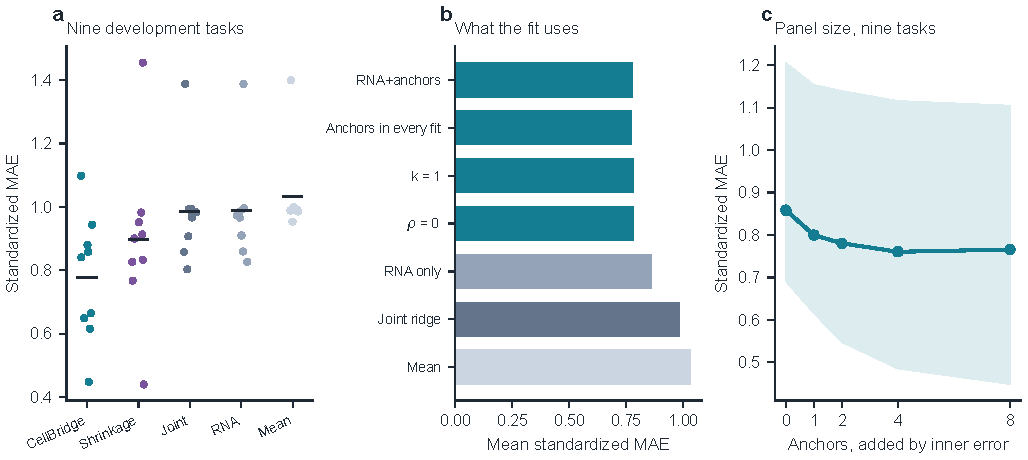
\includegraphics[width=174mm]{figure2_development.pdf}
\caption{AUTHOR: write this legend from OUTLINE.md. This is the development figure moved out of the main text.}
\label{fig:dev}
\end{figure*}
Alt text: Panel a is a strip plot of standardized error for five methods on nine development tasks. Panel b is a horizontal bar chart of the full model against ablations and two pseudobulk baselines. Panel c is a line with a shaded range showing error as the number of anchors grows from zero to eight. The shaded range is the minimum to the maximum across tasks.

\begin{figure*}
\centering
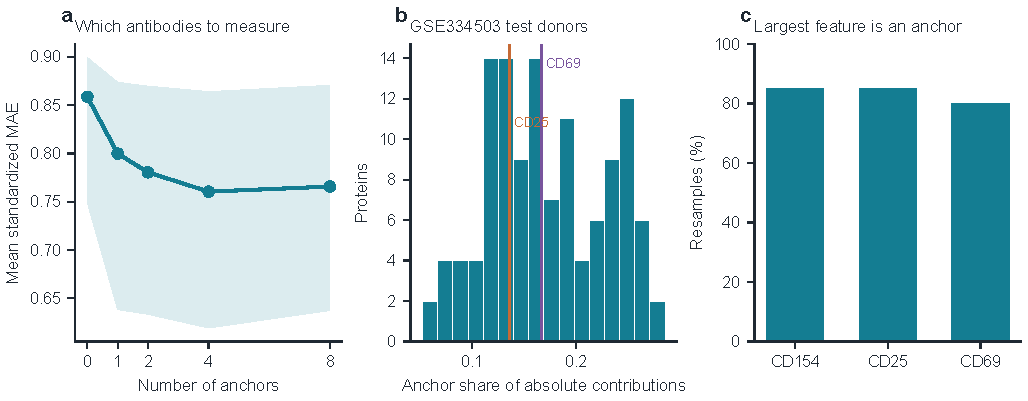
\includegraphics[width=174mm]{figure6_panel.pdf}
\caption{AUTHOR: write this legend from OUTLINE.md. This is the panel figure moved out of the main text.}
\label{fig:panel}
\end{figure*}
Alt text: Panel a shows mean error against the number of anchors, with an interquartile band. Panel b is a histogram of the share of absolute contribution coming from the eight anchors, with lines for CD25 and CD69. Panel c shows the percentage of bootstrap draws in which the largest feature is an anchor, for CD154, CD25 and CD69.

\begin{figure*}
\centering
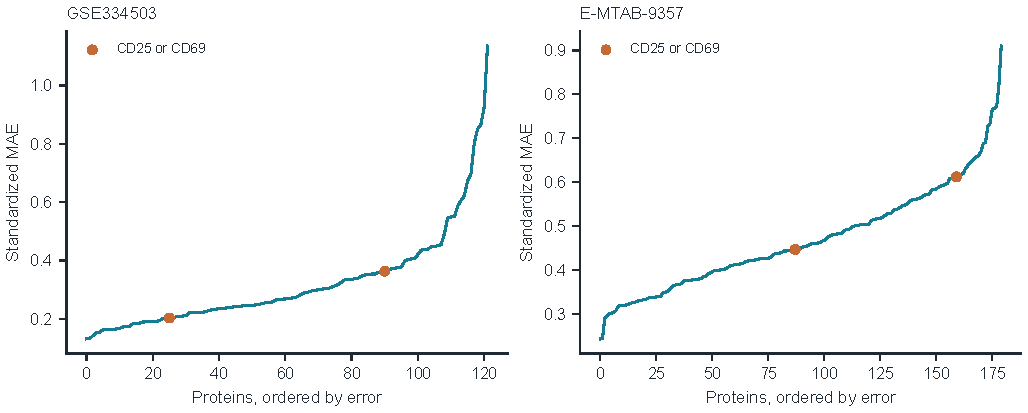
\includegraphics[width=174mm]{figureS1_per_protein.pdf}
\caption{AUTHOR: write this legend from OUTLINE.md.}
\label{fig:perprotein}
\end{figure*}
Alt text: Two curves, one per cohort, of standardized error with proteins ordered from smallest to largest error. CD25 and CD69 are marked.

\begin{figure*}
\centering
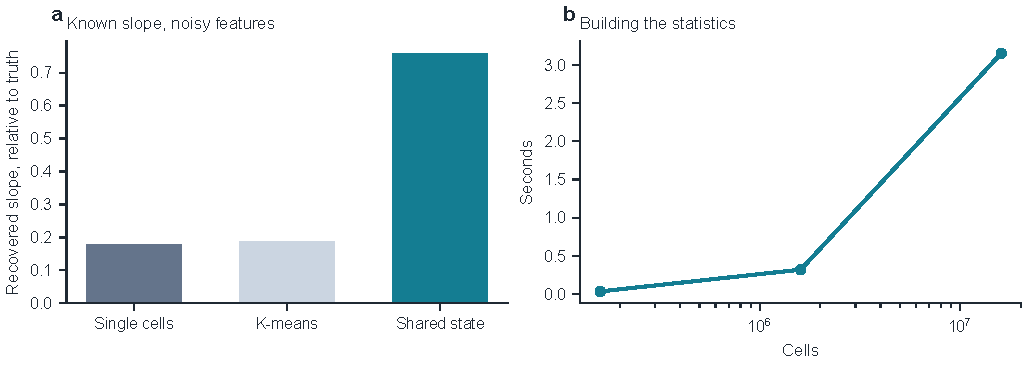
\includegraphics[width=174mm]{figureS2_simulation.pdf}
\caption{AUTHOR: write this legend from OUTLINE.md.}
\label{fig:simulation}
\end{figure*}
Alt text: Panel a compares recovered slope size for single cells, k-means and a shared state. Panel b shows seconds against the number of cells on a log axis.

\begin{figure*}
\centering
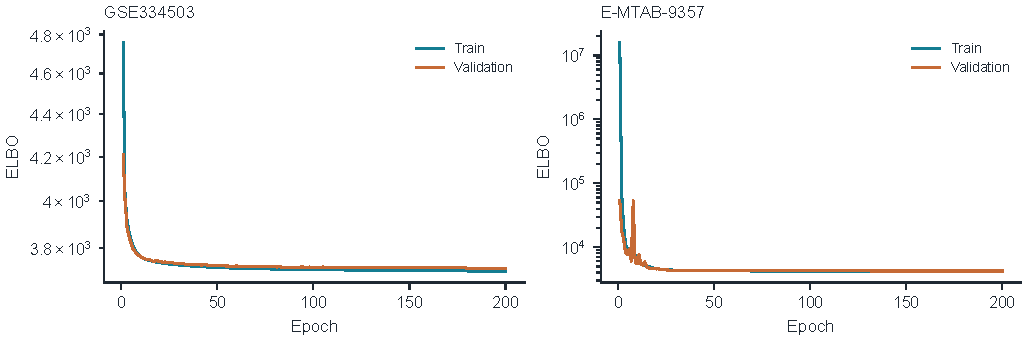
\includegraphics[width=174mm]{figureS3_totalvi.pdf}
\caption{AUTHOR: write this legend from OUTLINE.md.}
\label{fig:totalvi}
\end{figure*}
Alt text: Training and validation ELBO traces for the GSE334503 and E-MTAB-9357 totalVI fits, on a log axis.

\begin{figure}
\centering
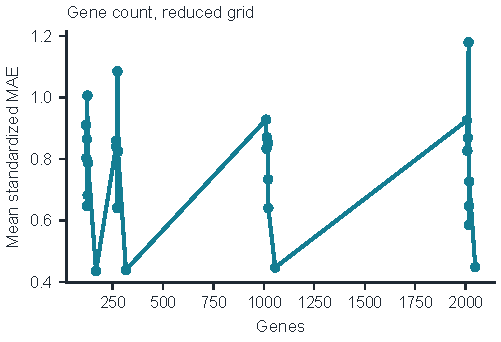
\includegraphics[width=85mm]{figureS4_genes.pdf}
\caption{AUTHOR: write this legend from OUTLINE.md.}
\label{fig:genes}
\end{figure}
Alt text: A line of mean standardized error against the number of genes on a reduced grid.

\end{document}
